\documentclass[tikz]{standalone}
\usepackage[utf8]{inputenc}
\usepackage{amsmath}
\definecolor{birugrafik}{RGB}{170,200,235}
\definecolor{birutebal}{RGB}{110,160,215}
\begin{document}
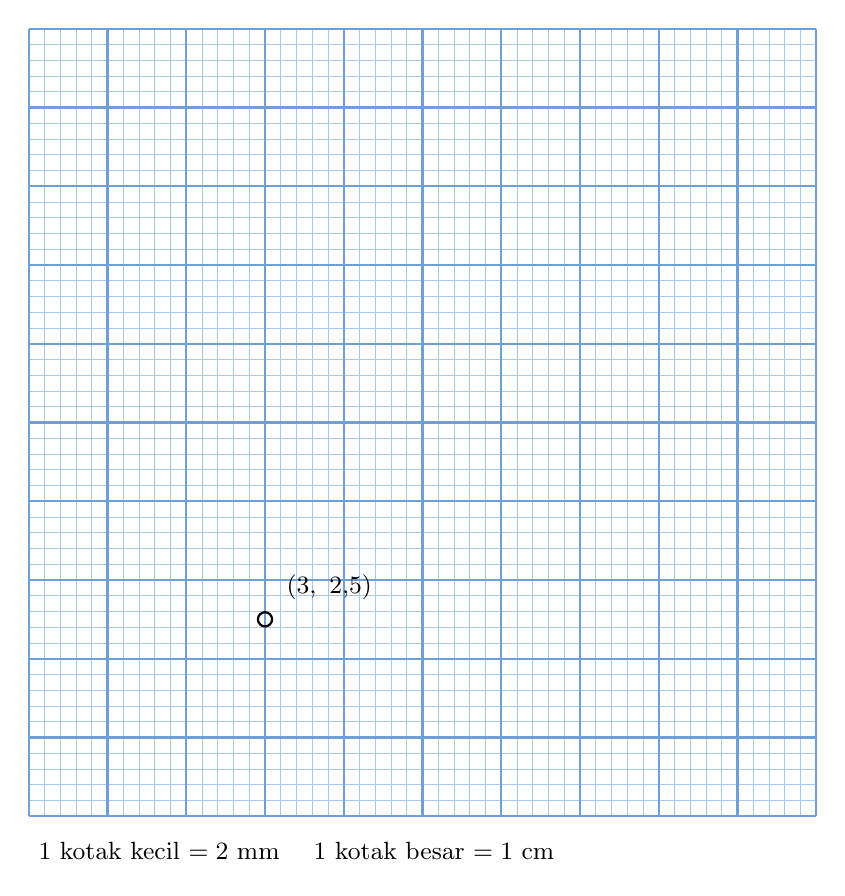
\begin{tikzpicture}[x=1cm,y=1cm]
  % garis tipis tiap 2 mm
  \foreach \i in {0,1,...,50}
    \draw[birugrafik, line width=0.3pt] (\i*0.2,0) -- (\i*0.2,10);
  \foreach \j in {0,1,...,50}
    \draw[birugrafik, line width=0.3pt] (0,\j*0.2) -- (10,\j*0.2);
  % garis tebal tiap 1 cm
  \foreach \k in {0,1,...,10}
    \draw[birutebal, line width=0.8pt] (\k,0) -- (\k,10);
  \foreach \k in {0,1,...,10}
    \draw[birutebal, line width=0.8pt] (0,\k) -- (10,\k);
  % label skala di bawah kertas
  \node[anchor=north west, font=\small] at (0,-0.2)
    {1 kotak kecil $=2$ mm \quad 1 kotak besar $=1$ cm};
  % contoh titik: (3 ; 2,5)
  \draw[black, thick] (3,2.5) circle (0.09);
  \node[anchor=south west, font=\small] at (3.15,2.62) {$(3,\ 2{,}5)$};
\end{tikzpicture}
\end{document}
